\chapter{Measuring Personal Clouds Services}

\section{Measurement Methodology}
During three months, we installed several
vantage points in our university network (\textit{Universitat
Rovira i Virgili}, Spain) and PlanetLab~\cite{planetlab}  
to measure the performance of three of the major Personal Cloud services in the market: DropBox\footnote{\url{http://www.dropbox.com}}, Box\footnote{\url{http://www.box.net}} 
and SugarSync\footnote{\url{http://www.sugarsync.com}}. The measurement methodology was based on the REST interfaces that these three Personal Cloud storage services provide to developers.

Personal Clouds provide REST APIs, along with
their client implementations, to make it possible for developers to
create novel applications. These APIs incorporate authorization
mechanisms (OAuth~\cite{oauth}) to manage the credentials and tokens
that grant access to the files stored in user accounts. A
developer first registers an application 
in the Cloud provider website and obtains several tokens.
As a result of this process, and once the user has authorized
that application to access his storage space, the Personal Cloud storage service
gives to the developer an \textit{access token}. Including this \textit{access token} in each API call, the application can operate on the user data.

There are two types of API calls: \textit{metadata-info} and
\textit{data management} calls. The former type refers to
those calls that retrieve information about the state of the
account (i.e., storage load, filenames), whereas the latter
are those calls targeted at managing the stored files
in the account. %In this work, 
We will analyze the performance
of the most important data management calls: \texttt{PUT} and \texttt{GET},
which serve to store and retrieve files.  


\subsection{Measurement Platform} 

We employed two different platforms
to execute our tests: University laboratories and PlanetLab.
The reason behind this is that our labs contain
\textit{homogeneous and dedicated machines} that are under our control,
while PlanetLab allows the analysis of each service from \textit{different geographic locations}. 

\textit{University laboratories}. We gathered $30$ machines
belonging to the same laboratory to perform the measurement.
These machines were Intel Core$2$ Duo equipped with $4$GB DDR$2$ RAM. 
The employed operating system was a Debian Linux distribution. 
Machines were internally connected to the same switch via a $100$Mbps Ethernet links.

\textit{PlanetLab}: We collected $40$ PlanetLab nodes divided into
two geographic regions: Western Europe and North America. 
This platform is constituted by heterogeneous (bandwidth, CPU) machines from several
universities and research institutes. Moreover, there were two points to consider
when analyzing data coming from PlanetLab nodes: i) Machines might be concurrently
used by other processes and users, and ii) The quota system of these machines
limited the amount of in/out data transferred daily. 

Specifically, we used the PlanetLab infrastructure for
a high-level assessment of Personal Clouds depending on the 
client's geographic location. 
However, the mechanisms to enforce bandwidth quotas
in PlanetLab nodes may induce the appearance of artifacts 
in bandwidth traces. This made PlanetLab not 
suitable for a fine-grained analysis in our context.
   
\begin{table}%
\begin{center}

\begin{tabular}{|l|l|l|l|}
\hline
Location & Op. Type & Operations & Transferred Data \\ \hline
\multirow{2}{*}{University Labs}
 & \texttt{GET} & $168,396$ & $13.509$ TB\\
 & \texttt{PUT} & $247,210$ & $15.945$ TB\\ \hline
\multirow{2}{*}{PlanetLab}
 & \texttt{GET} & $354,909$ & $31.751$ TB\\
 & \texttt{PUT} & $129,716$ & $9.803$ TB\\ \hline
\end{tabular}
\caption{Summary of Measurement Data (May $10$ $-$ July $15$)}
\vspace{-9mm}
\label{tab:measurement_data}
\end{center}
\end{table}

\subsection{Workload Model} 

Usually, Personal Cloud services impose file size 
limitations to their REST interfaces, for
we used only files of four sizes to facilitate comparison: $25$MB, $50$MB, 
$100$MB and $150$MB\footnote{Although the official limitation in some cases is fixed
to $300$MB per file, we empirically proved that uploading files
larger than $200$MB is highly difficult. In case of Box this limitation
is $100$MB.}. This approach provides an appropriate substrate 
to compare all providers with a large amount of samples of equal-size files.
Thanks to this, we could observe performance variations of a single provider
managing files of the same size.

In next sections we present the executed worloads.

\subsubsection*{Up/Down Workload}
The objective of this workload
was twofold: Measuring the maximum up/down transfer speed of operations
and detecting correlations between the transfer speed and the load
of an account. Intuitively, the first objective was achieved by alternating upload
and download operations, since the provider only needed to handle one 
operation per account at a time. We achieved the second point
by acquiring information about the load of an account in each API call.

The execution of this workload was continuously performed
at each node as follows: First, a node created synthetic 
files of a size chosen at random from the aforementioned set of sizes.
That node uploaded files until the capacity of the account was full.
At this point, that node downloaded all the files also in random order.
After each download, the file was deleted. 

\subsubsection*{Service Variability Workload}
This workload maintained 
in every node a nearly continuous upload and download transfer flow to analyze the performance 
variability of the service over time. This workload provides an
appropriate substrate to elaborate a time-series analysis of these services.

The procedure was as follows: The upload process first
created files corresponding to each defined file size which
were labeled as ``reserved'', since they were not deleted from the account.
By doing this we assured that the download process was never interrupted,
since at least the reserved files were always ready for being downloaded.
Then, the upload process started uploading synthetic 
random files until the account was full. When the account was full,
this process deleted all files with the exception of the reserved ones
to continue uploading files.
In parallel, the download process was continuously downloading random files
stored in the account. 
 
Finally, we executed the experiments
in different ways depending on the chosen platform. In the case of
PlanetLab, we employed the \textit{same machines in each test}, and therefore, 
we needed to sequentially execute all the combinations of workloads and providers. 
This minimized the impact of hardware and network
heterogeneity, since all the experiments were executed in the same conditions.
On the contrary, in our labs we executed in parallel a certain workload
for all providers (i.e. assigning $10$ machines per provider).
This provided two main advantages: The measurement process was
substantially faster, and fair comparison of the three services
was possible for the same period of time. 
 
We depict in Table \ref{tab:measurement_data} the total 
number of storage operations performed during the measurement period.

\subsection{Setup, Software and Data Collection}

Prior to the start of our experiments, we created 
around $150$ new user free accounts from the targeted Personal Clouds.
That is $120$ new accounts for PlanetLab experiments ($40$ nodes
$\times$ $3$ Personal Clouds), and $30$ accounts for the experiments
in our labs ($10$ accounts per Personal Cloud deployed in $30$ machines). 
We also registered as developers $35$ applications to access the storage
space of user accounts via REST APIs, obtaining the necessary tokens
to authenticate requests.
We assigned to every node a single new free account with access permission
to the corresponding application.
The information of these accounts was stored in a database hosted in our research servers.
Thus, nodes executing the measurement process were able to access the
account information remotely. 

Measurement processes were implemented as
Unix and Python scripts that ran in every node. These scripts employed
third party tools during their execution. For instance, to synchronize tasks, 
such as logging and starting/finishing
experiments, we used the \texttt{cron} time-based job scheduler.
To gather bandwidth information we used
\texttt{vnstat}, %\footnote{\url{http://humdi.net/vnstat/}}: 
a tool that keeps a log of network 
traffic for a selected interface. Nodes performed storage operations against Personal Clouds 
thanks to the API implementations released in their websites. 

The measurement information collected in each storage operation
was sent periodically from every node 
to a database hosted in our research servers. This automatic process
facilitated the posterior data processing and exploration. The measurement information
that nodes sent to the database describes several aspects of the service performance:
operation type, bandwidth trace, file size, start/end time instants, 
time zone, capacity and load of the account, and failure information.

\section{Results}

\subsection{Transfer Capacity of Personal Clouds}
%Transfer characterization: avg. transfer distributions, bandwidths distributions, times
%Service variability depending on the day of the week
In this section, the transfer capacity of Box, DropBox and SugarSync is characterized using the following indicators:
\begin{itemize}
	\item \textit{File Mean Transfer Speed (MTS)}. This metric is defined as \textit{the ratio of
	the size of a file, $S$, to the time, $T$, that was spent to transfer it: $MTS = {S}/{T}$ (KBytes/sec)}. 
	\item \textit{Bandwidth Distributions}. We define as a \textit{bandwidth trace} the set of
	values that reflects the transfer speed of a file at regular intervals of $2$ secs. To
	obtain a single empirical distribution, we aggregated the bandwidth traces of
	all the transfers separated by uploads and downloads. We refer to the resulting empirical
	distribution as the \textit{aggregated bandwidth distribution}.
	 
\end{itemize}

\subsubsection*{Transfer speeds}
Fig.~\ref{fig:transfer_mean_speeds_and_bw_distributions} 
reports these metrics for both workloads (up/down and service
variability) executed in our university labs during $10$ days.
First, Fig.~\ref{fig:transfer_mean_speeds_and_bw_distributions} 
evidences an interesting fact: \textit{Personal Clouds 
are heterogeneous in terms of transfer speed}.
For instance, Fig.~\ref{fig:avg_up_file_transfer_speed} 
shows that Box and DropBox present an upload MTS 
several times faster than SugarSync. The same observation holds for
downloads. Moreover, the heterogeneity of these services also depends
on the \textit{traffic type} (in/out). This can be appreciated by
comparing Fig.~\ref{fig:avg_down_file_transfer_speed} 
with Fig.~\ref{fig:avg_up_file_transfer_speed}: \textit{DropBox exhibits
the best download MTS while Box presents the fastest 
uploads.}

This proves that \textit{the transfer performance of these services greatly varies among providers}, and
consequently, developers should be aware of this in order to select an adequate provider. 

Among the examined Personal Clouds, DropBox and SugarSync 
are \textit{resellers} of major Cloud storage providers (Amazon S3 
and Carpathia Hosting, respectively). On the other hand, Box claims to be owner of several
datacenters. In our view, it is interesting to analyze this 
Cloud ecosystem and the possible implications to the service delivered to end-users.

\begin{figure}[t]
  \subfigure[Download file MTS distributions.]
{\label{fig:avg_down_file_transfer_speed}
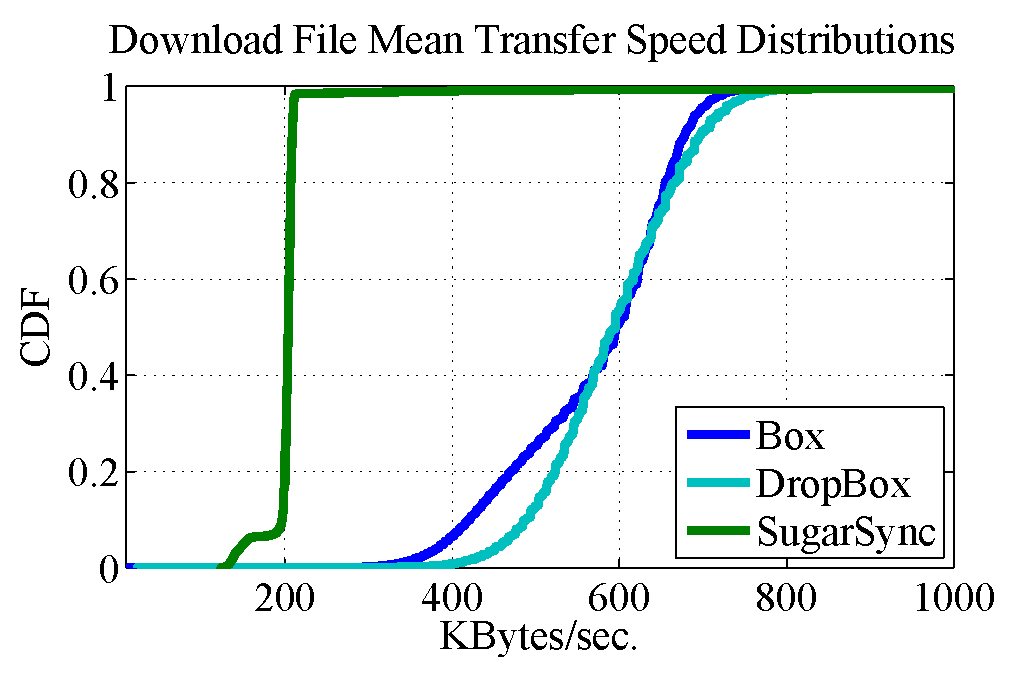
\includegraphics[width=0.5\textwidth]{figures/avg_down_file_transfer_speed_new.eps}}
  \subfigure[Upload file MTS distributions.]
{\label{fig:avg_up_file_transfer_speed}
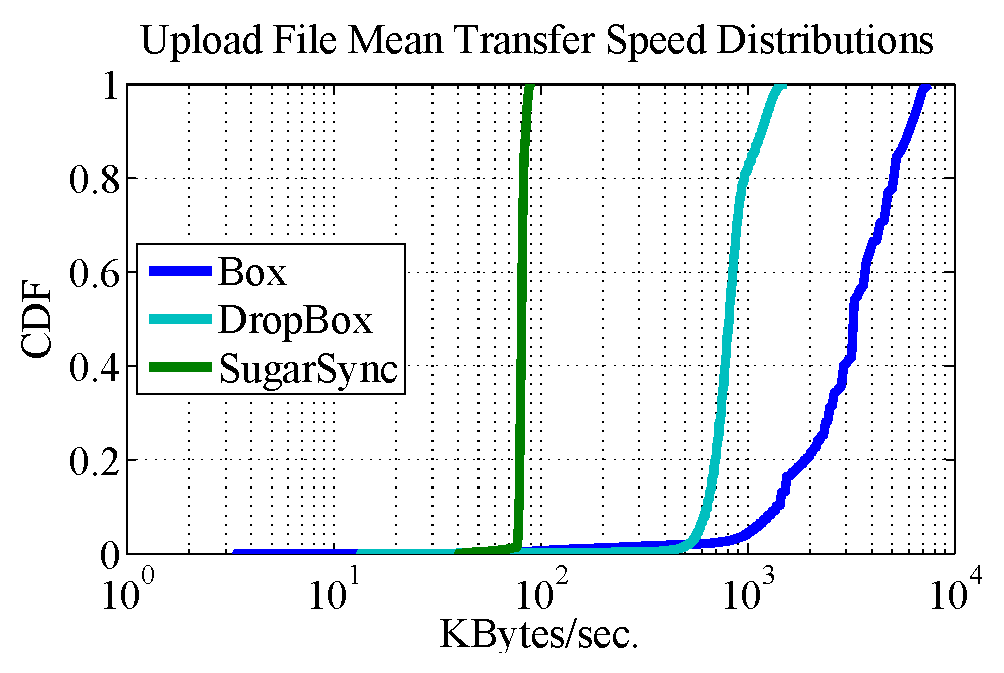
\includegraphics[width=0.5\textwidth]{figures/avg_up_file_transfer_speed_new.eps}}      
  \subfigure[Download bandwidth distributions.]
{\label{fig:down_bw_comparison}
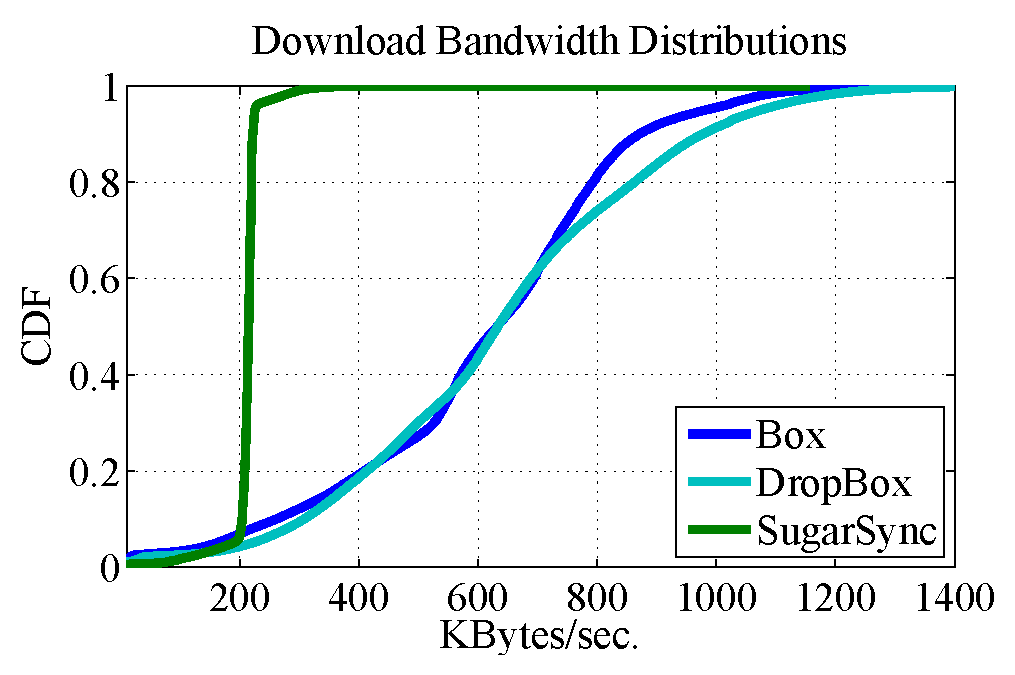
\includegraphics[width=0.5\textwidth]{figures/down_bw_comparison_new.eps}}
  \subfigure[Upload bandwidth distributions.]
{\label{fig:up_bw_comparison}
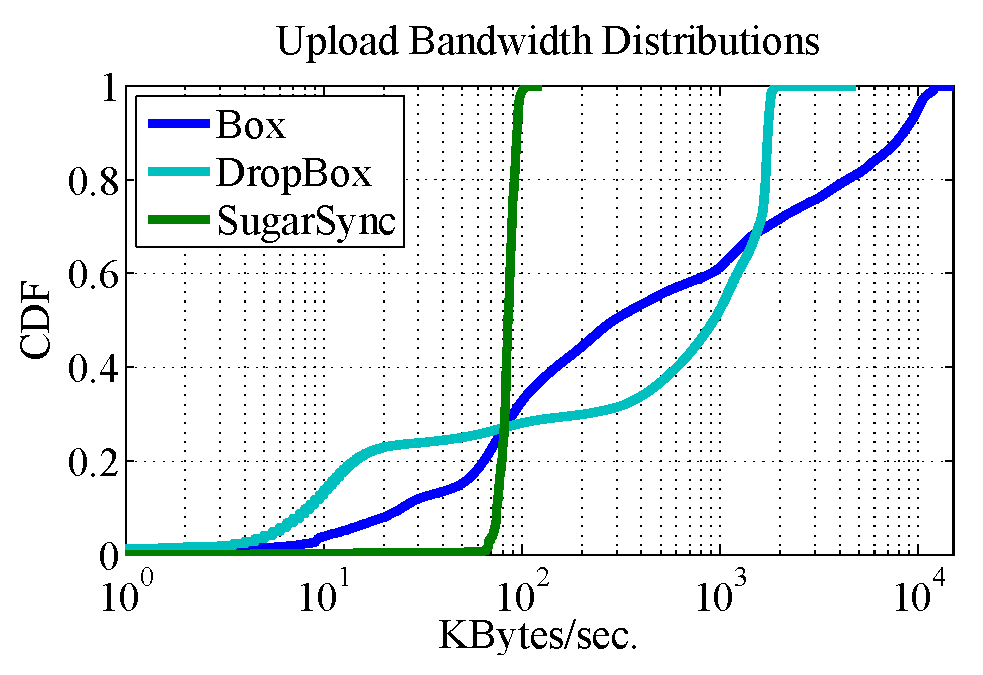
\includegraphics[width=0.5\textwidth]{figures/up_bw_comparison_new.eps}}
 
   \caption{Transfer capacity of Box, DropBox and SugarSync free account REST API services.
   The data represented in these figures corresponds to the aggregation
   of the up/down and service variability workloads during $10$ days (June/July $2012$) in our university laboratories.}
   \label{fig:transfer_mean_speeds_and_bw_distributions}
   \vspace{-4mm}
\end{figure}

In this sense, in Fig. \ref{fig:transfer_mean_speeds_and_bw_distributions} we observe  
that Personal Clouds apply \textit{distinct internal control policies}
to the inbound/outbound bandwidth provided to users. To wit,
both DropBox and Box exhibit an \textit{upload transfer capacity remarkably better
than the download capacity}. This means that the datacenter outgoing
traffic is more \textit{controlled and restricted} than the incoming traffic. This agrees
well with the current pricing policies of major Cloud providers (Amazon S3,
Google Storage) which do not charge inbound traffic whereas
the outbound traffic is subject to specific rates (see \url{http://aws.amazon.com/en/s3/pricing/}). 

In SugarSync, both the upload and download transfer speeds are constant and
low. Interestingly, SugarSync presents slightly faster downloads than uploads,
though only a small fraction of downloads (less than $1\%$) exhibits a much
higher transfer speed than the rest. These observations are also supported by Fig.~\ref{fig:down_bw_comparison} and Fig.~\ref{fig:up_bw_comparison}: the captured download
bandwidth values fall into a small range $[200, 1300]$ KB/sec. Also,
the shape of these distributions are not steep, which reflects that there is
a strong control in the download bandwidth.
On the contrary, upload bandwidth distributions present more irregular shapes and
they cover a wider range of values, specially for Box.
As a possible explanation to this behavior, the experiments of Fig. \ref{fig:transfer_mean_speeds_and_bw_distributions} 
were executed from our university labs (Spain) to exclude the impact of geographic heterogeneity. 
Considering the fact that the majority of 
Personal Cloud datacenters are located in USA~\cite{drago2013benchmarking}, 
this may have implications in the cost of the traffic sent to Europe. This could motivate
the enforcement of more restrictive bandwidth control policies to
the outbound traffic.
\medskip

\subsubsection*{Transfers \& geographic location}. 
Next, we analyze transfer speeds depending
on the geographic location of vantage points. 

In Fig.~\ref{fig:transfer_times_geographic_location},
we illustrate the file MTS obtained from executing the up/down 
workload during $3$ weeks in PlanetLab. 
As can be seen in the figure, \textit{Personal Clouds provide a
much greater QoS in North American countries than in European countries}.
Intuitively, the location of the datacenter plays
a critical role in the performance of the service delivered to users. 
Observe that this phenomenon is orthogonal to all the examined vendors.

Finally, we quantify the relative download/upload transfer performance delivered by 
each service as a function of the geographic location of users.
To this end,
we used a simple metric, what we call the \textit{download/upload ratio} ($D/U$), which
is the result of dividing the download and upload transfer speeds of a certain vendor.   
In Table \ref{tab:down_up_ratio_location}, we calculated this ratio over the mean ($\bar{U},\bar{D}$) 
and median ($\tilde{U},\tilde{D}$) values of the file MTS distributions of each
provider depending on the geographic location of nodes. 

In line with results obtained in our university labs, 
\textit{European nodes receive a much higher 
transfer speed when uploading than when downloading} ($D/U<1$). 
However, contrary to conventional wisdom, \textit{North American nodes exhibit 
just the opposite behavior}. This is clearly visible in DropBox and Box. However, this ratio is constant
in SugarSync, irrespective of the geographic location.



\begin{figure}[h]
\centering	
{\label{fig:transfer_times_geographic_location_downloads}
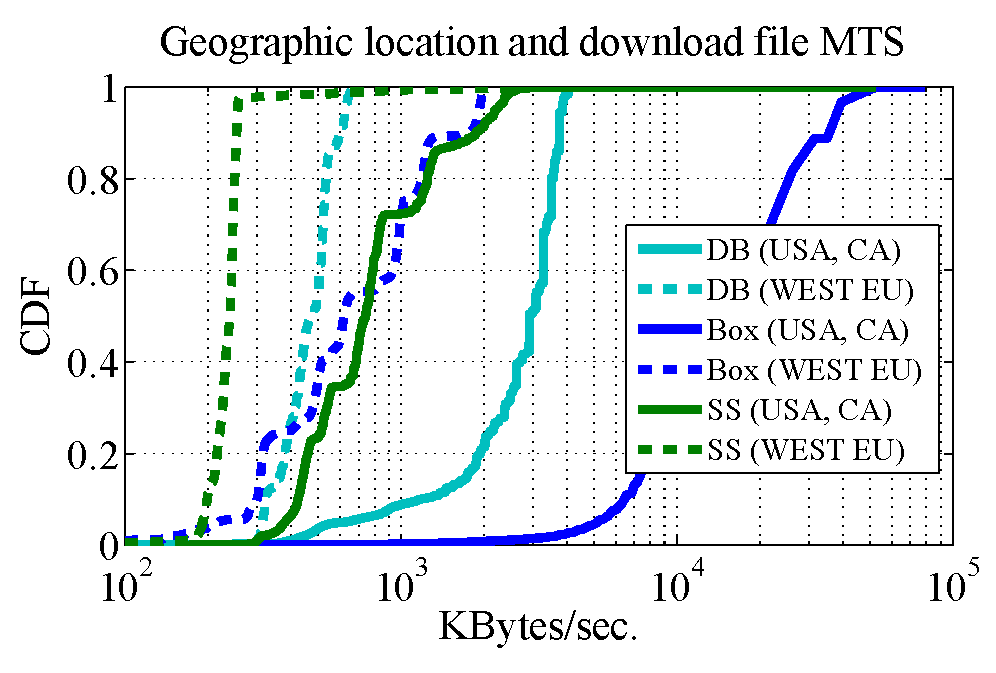
\includegraphics[width=0.48\textwidth]{figures/geographic_location_downloads.eps}} 
{\label{fig:transfer_times_geographic_location_uploads}
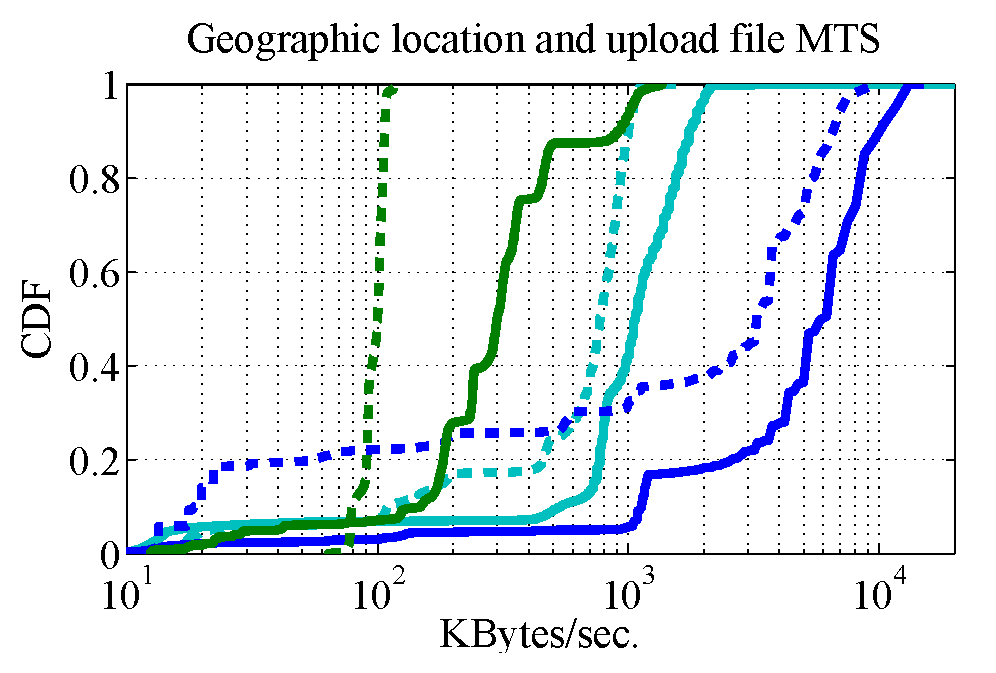
\includegraphics[width=0.48\textwidth]{figures/geographic_location_uploads.eps}}
%\subfloat[-.]
%{\label{fig:mean_upload_speed_distributions_by_file_size}
%\includegraphics[width=0.24\textwidth]{mean_upload_speed_distributions_by_file_size.eps}}
%  \subfloat[-.]
%{\label{fig:mean_download_speed_distributions_by_file_size}
%\includegraphics[width=0.24\textwidth]{mean_download_speed_distributions_by_file_size.eps}} 
	\caption{File MTS distributions of PlanetLab nodes from June $22$ to July $15$ 
	$2012$ depending on their geographic location (up/down workload).
	Clearly, USA and Canada nodes exhibit faster transfers than European nodes.}
	\label{fig:transfer_times_geographic_location}
	%\vspace{-1mm}
\end{figure}


\begin{table}[h]
\begin{center}
\begin{tabular}{|l|l|l|l|l|}
\hline
 Geo. Location& \textit{Metric} & Box & DropBox & SugarSync \\ \hline
\multirow{2}{*}{USA \& CA}
 & $\bar{D}_{MTS}/\bar{U}_{MTS}$ & $3.198$ & $2.482$ & $2.522$ \\
 & $\tilde{D}_{MTS}/\tilde{U}_{MTS}$ & $2.550$ & $2.722$ & $2.500$ \\ \hline
\multirow{2}{*}{WEST EU}
 & $\bar{D}_{MTS}/\bar{U}_{MTS}$ & $0.255$ & $0.681$ & $2.589$ \\
 & $\tilde{D}_{MTS}/\tilde{U}_{MTS}$ & $0.190$ & $0.682$ & $2.387$ \\ \hline
\end{tabular}
\caption{Download/Upload transfer speed ratio of Personal Clouds depending on the client's geographic location.}
\vspace{-5mm}
\label{tab:down_up_ratio_location}
\end{center}
\end{table}

\begin{figure}
\centering	
	\subfigure[Download transfer times CDF.]{
  		\label{fig:down_transfer_times_by_size}
		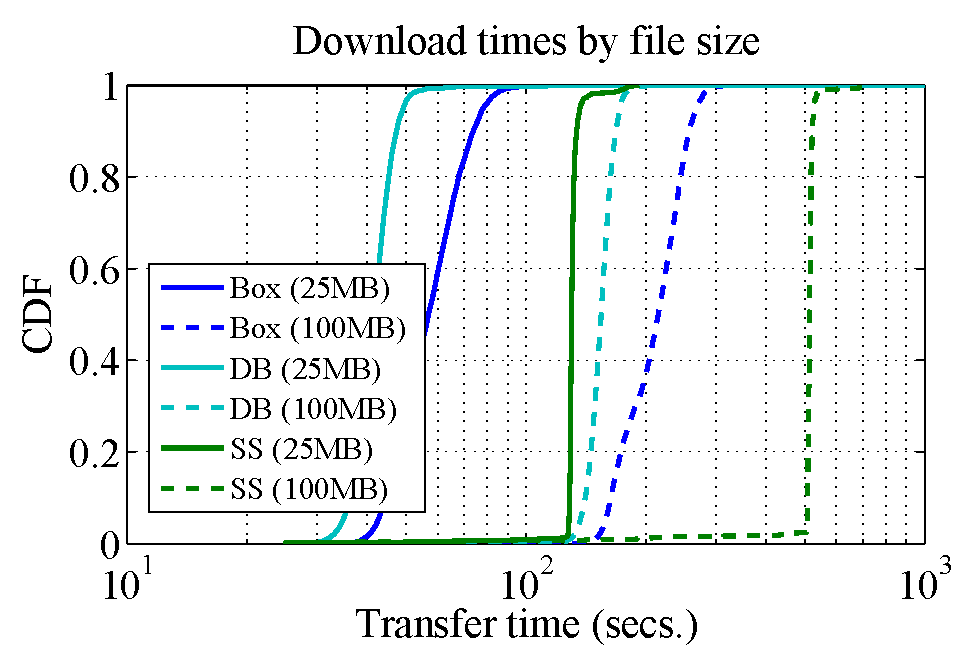
\includegraphics[width=0.45\textwidth]{figures/download_times_by_file_size.eps}
	}
 	\subfigure[Upload transfer times CDF.]{
 		\label{fig:up_transfer_times_by_size}
 		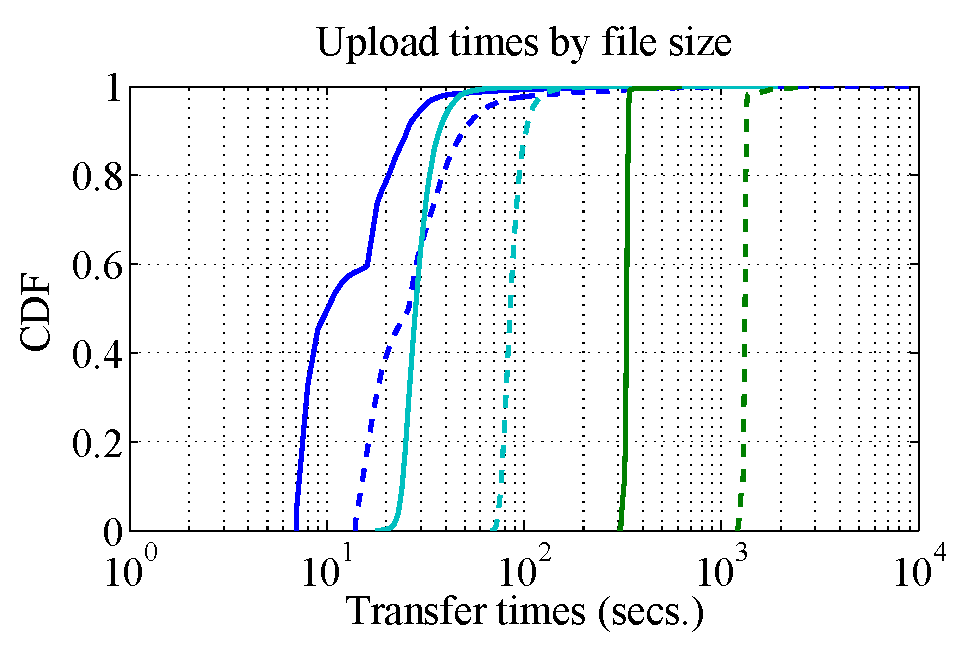
\includegraphics[width=0.45\textwidth]{figures/upload_times_by_file_size.eps}
 	}
	\caption{Transfer times distributions by file size.}
	\label{fig:transfer_times_and_speed_by_size}
	%\vspace{-4mm}
\end{figure}


\begin{table*}[t]
%\hspace*{-40mm}
\renewcommand{\arraystretch}{1}\addtolength{\tabcolsep}{-3pt}
\tiny
\centering
\begin{tabular}{|p{0.65cm}|c|c|c|c|c|c|c|c|c|}
\hline

& & \multicolumn{8}{|c|}{Download File MTS Distribution (KBps)} \\

\hline
Size 		& Provider & Min. & Q1 & Median & Q3 & Max. & Mean ($\mu$) & Std. Dev. ($\sigma$) & CV ($\sigma/\mu$) \\ \hline
\multirow{3}{*}{$25$MB} 
 & DropBox & $24.89$ & $582.54$ & $624.152$ & $672.16$ & $970.90$ & $626.94$ & $71.23$ & $0.1136$  \\
 & Box & $163.84$ & $397.19$ & $459.90$ & $534.99$ & $794.38$ & $463.72$ & $87.76$ & $0.0837$  \\
 & SugarSync & $136.53$ & $198.59$ & $200.11$ & $201.65$ & $1048.57$ & $201.35$ & $37.89$ & $0.1882$  \\ \hline
 								
\multirow{3}{*}{$50$MB} 
 & DropBox & $210.56$ & $624.15$ & $663.66$ & $699.05$ & $888.62$ & $661.55$ & $58.02$ & $0.0877$   \\
 & Box & $14.15$ & $623.16$ & $647.26$ & $672.16$ & $887.42$ & $646.22$ & $44.33$ & $0.0686$  \\
 & SugarSync & $144.43$ & $200.88$ & $202.43$ & $204.00$ & $2496.61$ & $216.57$ & $149.28$ & $0.6893$  \\ \hline
 								
\multirow{3}{*}{$100$MB} 
 & DropBox & $25.09$ & $647.27$ & $676.50$ & $708.49$ & $1497.97$ & $680.32$ & $50.94$ & $0.0749$  \\
 & Box & $14.43$ & $436.91$ & $487.71$ & $579.32$ & $1233.62$ & $507.82$ & $89.36$ & $0.0539$  \\ 
 & SugarSync & $145.64$ & $202.03$ & $204.00$ & $205.20$ & $3744.91$ & $223.49$ & $219.50$ & $0.9822$  \\ \hline
 
\end{tabular}
\caption{Summary of download file MTS distributions by file size.}
\label{tab:service_variability_file_size_download}
\end{table*}


\subsection{Variability of Transfer Performance}
\label{sec:variability}

In this section, we analyze which factors can contribute to the
variance in transfer speed observed in Personal Clouds.~We
study three potential factors, which are \textit{the size of file transfers};
\textit{the load of accounts}; and \textit{time-of-day effects}.
\medskip

%<<<<<<< .mine
%\textbf{Transfers \& file size}. Regarding the first question, we analyze the role of the
%file size in the API service based on \textit{transfer times} 
%=======
\subsubsection*{Variability over file size}.
We first investigate the role that 
file size plays on \textit{transfer times} 
%>>>>>>> .r818
and \textit{transfer speeds}. Fig. \ref{fig:transfer_times_and_speed_by_size}
and Tables \ref{tab:service_variability_file_size_download} and \ref{tab:service_variability_file_size_upload} report the results
for both metrics as function of file size, respectively. Unless otherwise
stated, results reported in this subsection are based on executing the 
up/down workload in our university labs during $5$ days.  

Fig. \ref{fig:transfer_times_and_speed_by_size} plots the
transfer time distribution for all the evaluated
Personal Clouds. As shown in the figure, for
the same provider, all the distributions present a similar
shape, which suggests that \textit{the size of file transfers is not a 
source of variability}. As expected, the only difference is that
the distributions for large file sizes are shifted to the right towards
longer time values. Significant or abnormal differences were not observed
when transferring large files compared to small data files. This observation is applicable to all evaluated Personal Clouds. 
This leads us to the conclusion that these Personal Clouds
\textit{do not perform aggressive bandwidth throttling policies to large files}.

An interesting fact appreciable in Tables \ref{tab:service_variability_file_size_download} and \ref{tab:service_variability_file_size_upload}
is that \textit{managing larger files report better transfer 
speeds than in case of small files}. Usually, these 
improvements are slight or moderate ($0.5\%$ to $25\%$ higher MTS); 
however, uploading $100$MB files to Box exhibits a MTS $48\%$ higher
than uploading $25$MB files to this service. In our view, this phenomena is due
to the variability in the incoming bandwidth supplied by Box, and 
the TCP slow start mechanism, which makes difficult for small file transfers 
to attain high performance~\cite{allman1999tcp}. 

Further, we found that all the measured Cloud vendors tend to perform a more restrictive
bandwidth control to outgoing traffic. This can be easily confirmed
by inspecting the obtained standard deviations $\sigma$ of file MTS 
listed in Table \ref{tab:service_variability_file_size_download}. Clearly,
\textit{the inbound traffic in Dropbox and Box is much more variable than the outbound traffic}. 
On the contrary, despite its limited capacity, the source of highest
transfer variability in SugarSync is in the outbound traffic, which a clear
proof of the existing heterogeneity in Personal Clouds.


\begin{table*}[t]
%\hspace*{-40mm}
\renewcommand{\arraystretch}{1}\addtolength{\tabcolsep}{-3pt}
\tiny
\centering
\begin{tabular}{|p{0.65cm}|c|c|c|c|c|c|c|c|c|}
\hline

& & \multicolumn{8}{|c|}{Upload File MTS Distribution (KBps)} \\

\hline
Size 		& Provider & Min. & Q1 & Median & Q3 & Max. & Mean ($\mu$) & Std. Dev. ($\sigma$) & CV ($\sigma/\mu$) \\ \hline
\multirow{3}{*}{$25$MB} 
 & DropBox & $13.54$ & $819.20$ & $903.94$ & $1008.24$ & $1456.36$ & $896.28$ & $151.56$ & $0.1691$  \\
 & Box & $14.70$ & $1379.71$ & $2383.13$ & $3276.80$ & $3744.91$ & $2271,29$ & $973.06$ & $0.3963$  \\
 & SugarSync & $41.87$ & $78.25$ & $78.96$ & $80.17$ & $86.23$ & $79.26$ & $2.82$ & $0.0356$  \\ \hline
 								
\multirow{3}{*}{$50$MB} 
 & DropBox & $213.99$ & $970.90$ & $1092.27$ & $1191.56$ & $1497.97$ & $1069.12$ & $152.23$ & $0.1424$  \\
 & Box & $5.26$ & $2496.61$ & $4369.07$ & $4766.25$ & $5825.42$ & $3721.12$ & $1357.18$ & $0.3647$  \\
 & SugarSync & $40.27$ & $78.72$ & $79.44$ & $80.41$ & $86.95$ & $79.59$ & $3.08$ & $0.0387$  \\ \hline
 								
\multirow{3}{*}{$100$MB} 
 & DropBox & $250.26$ & $1127.50$ & $1219.27$ & $1310.72$ & $1519.66$ & $1205.69$ & $143.05$ & $0.1186$  \\
 & Box & $4.71$ & $2912.71$ & $3883.61$ & $6168.09$ & $7489.83$ & $4350.37$ & $1797.32$ & $0.3252$  \\ 
 & SugarSync & $42.23$ & $78.96$ & $79.62$ & $80.66$ & $87.31$ & $79.64$ & $3.74$ & $0.0470$  \\ \hline
 
\end{tabular}
\caption{Summary of upload file MTS distributions by file size.}
\label{tab:service_variability_file_size_upload}
\end{table*}

\begin{figure}[t]
\center
  \subfigure[SugarSync does not present important changes
  in both in/out traffic speed over time.]
{\label{fig:transfer_time_series_variability_sugarsync}
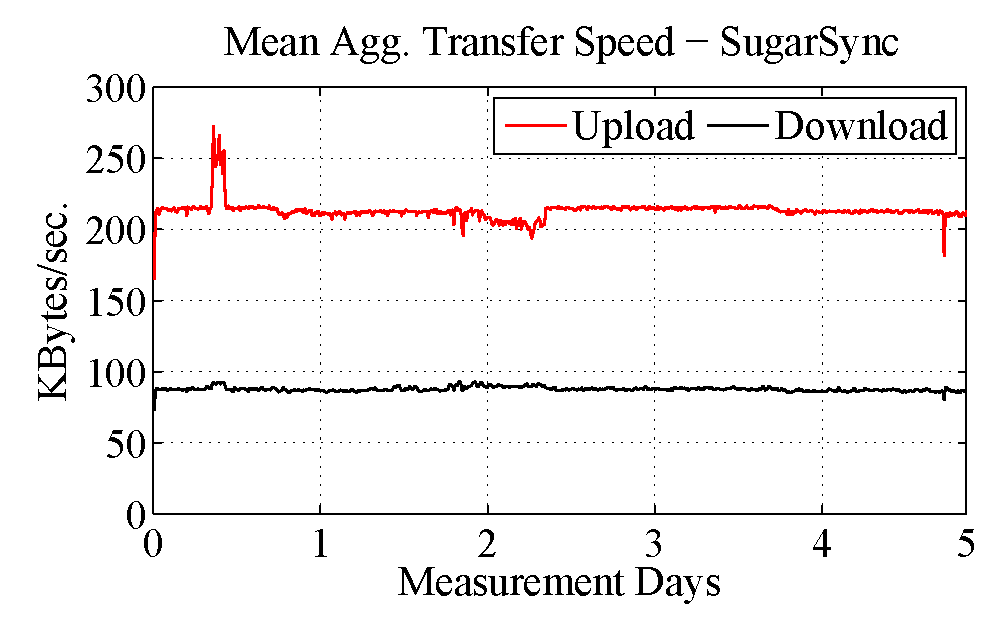
\includegraphics[width=0.45\textwidth]{figures/sugarsync_time_series.eps}}
  \subfigure[We observe daily patterns in the DropBox upload transfer speed.
  Download transfer speed remains stable.]
{\label{fig:transfer_time_series_variability_dropbox}
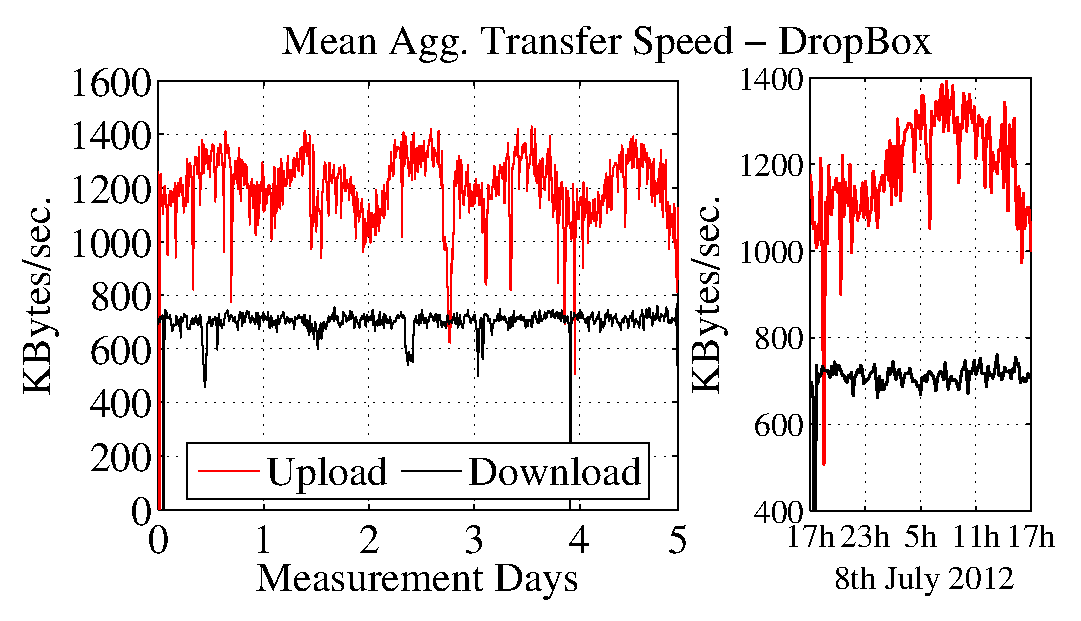
\includegraphics[width=0.45\textwidth]{figures/dropbox_time_series.eps}}  
  \subfigure[Box upload transfers are highly variable and probably affected by
  daily patterns.]
{\label{fig:transfer_time_series_variability_box}
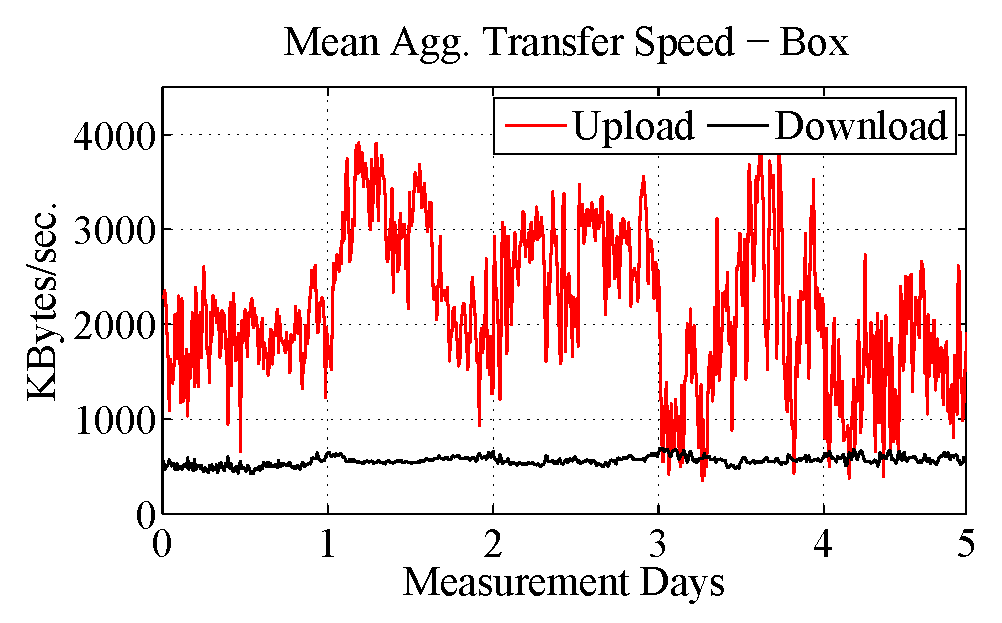
\includegraphics[width=0.45\textwidth]{figures/box_time_series.eps}}         
   \caption{Evolution of Personal Clouds upload/download transfer speed during $5$ days. We plotted
   in a time-series fashion the mean aggregated bandwidth of all nodes ($600$ secs. time-slots) executing 
   the service variability workload in our university laboratories ($3$rd$-8$th July $2012$).}
   \label{fig:transfer_time_series_variability}
	\vspace{-3mm}
\end{figure}


\medskip

\subsubsection*{Variability over time}. We now analyze how the
transfer speed varies over time. To better capture these variations, 
we used the data from the \textit{service variability workload}, 
which was aimed to maintain a constant transfer flow and was executed at our university labs.
The results are shown in Fig. \ref{fig:transfer_time_series_variability} 
where the \textit{mean aggregated bandwidth} of all nodes as a whole is plotted in time 
intervals~of $600$ seconds. As expected, we found that the transfer speed of these services behave
differently depending on the provider.~To wit, while SugarSync
exhibits a \textit{stable service for both uploads and downloads}, at
the price of a modest transfer capacity (Fig. \ref{fig:transfer_time_series_variability_sugarsync}), the upload transfer
speed varies significantly over time for Dropbox and Box.

%As depicted in Fig. 
Appreciably, \textit{DropBox exhibits appreciable 
daily upload speed patterns} (Fig. \ref{fig:transfer_time_series_variability_dropbox}). 
Data represented in Fig. \ref{fig:transfer_time_series_variability} was gathered between
July $3$, $6$:$00$p.m. and July $8$, $3$:$00$p.m. Clearly, during 
night hours ($1$ a.m.$-10$ a.m.), transfer speed was between $15\%$ to
$35\%$ higher than during diurnal hours. This phenomenon has been also
detected in the experiments performed in PlanetLab, thereby discarding
any artificial usage pattern induced by our university network. Moreover, considering
that DropBox uses Amazon S3 as storage backend, our results are consistent with
other recent works~\cite{variability_ccgrid11} that observed 
similar patterns in other Amazon services.

Further, we found that Box upload service may be subjected to
high variability over time. Indeed, we observed \textit{differences in
upload transfer speed by a factor of $5$  along the same day}. This observation is consistent 
with the analysis of the file MTS distribution where significant
heterogeneity was present. More interestingly, Box uploads 
appear to be also affected by \textit{daily patterns}. Concretely, 
the periods of highest upload speed occurred during
the nights, whereas the lowest upload speeds were observed during the
afternoons ($3$ p.m. $-10$ p.m.). Due to the huge variability
of this service, a long-term measurement is needed to provide
a solid proof of this phenomenon, though.


With respect to downloads, we observed no important
speed changes over time in any system. This suggests that
\textit{downloads are more reliable and predictable, probably
due to a more intense control of this type of traffic by
the datacenter}.